\subsection{Raytracing}
\begin{wrapfigure}{r}{0.3\linewidth}
\centering
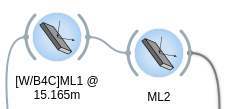
\includegraphics[width=0.3\textwidth]{images/DMM_oasys.png}
\caption{\label{fig:DMM_oasys} Double Multilayer Monochromator in Oasys Shadow.}
\end{wrapfigure}

The double-bounce DMM is modelled with two Shadow Plane Mirror widgets in series (Figure \ref{fig:DMM_oasys}). ML reflectivity is modelled with a Shadow PreMLayer widget as shown in Figure \ref{fig:PreMLayer}. The mirror surface is modified with Surface Error external splines with varying longitudinal slope error (0.1, 0.2, 0.3, 0.4 and 0.5 $\mu rad$ RMS). These modified surfaces (\ref{fig:fractals}) are simulated with the Shadow PreProcessor - Height Profile Simulator widget. The transversal slope error is kept constant at 20 $\mu rad$ RMS and fractal profiles are chosen. 

\begin{figure}  % spans both columns
\begin{subfigure}{0.5\textwidth}
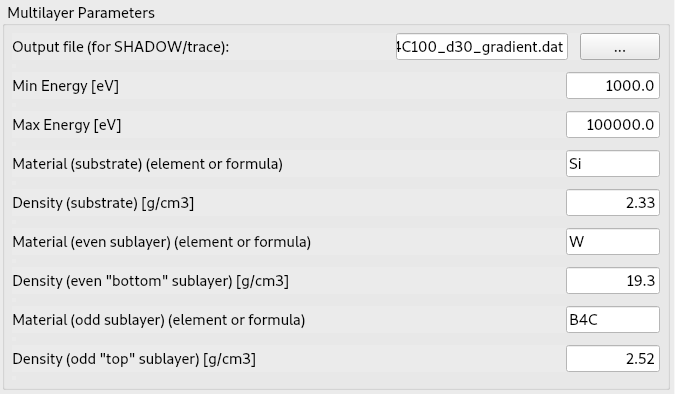
\includegraphics[width=\linewidth]{images/MLspecs_a.png}
\end{subfigure}
\hfill % maximize the horizontal distance between the graphs
\begin{subfigure}{0.5\textwidth}
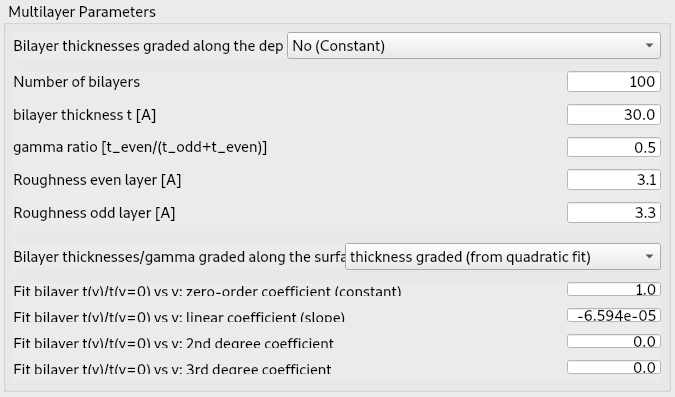
\includegraphics[width=\linewidth]{images/MLspecs_b.png}
\end{subfigure}
\caption{\label{fig:PreMLayer} PreMLayer widget settings in Shadow. }
\end{figure}

\begin{figure}[!htb]
\minipage{0.32\textwidth}
  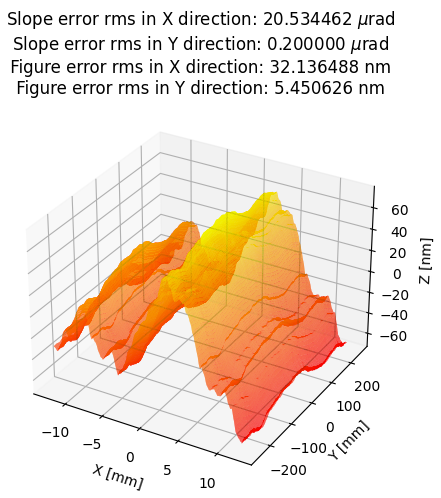
\includegraphics[width=\linewidth]{./../figures/slope_error/surface_error_profile_500x25_02x20urad.png}
  % \caption{A really Awesome Image}\label{fig:awesome_image1}
\endminipage\hfill
\minipage{0.32\textwidth}
  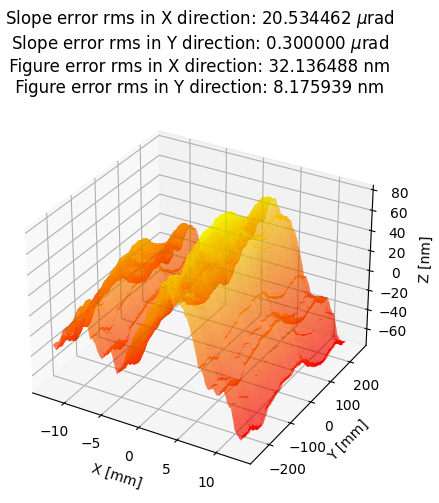
\includegraphics[width=\linewidth]{./../figures/slope_error/surface_error_profile_500x25_03x20urad.png}
  % \caption{A really Awesome Image}\label{fig:awesome_image2}
\endminipage\hfill
\minipage{0.32\textwidth}%
  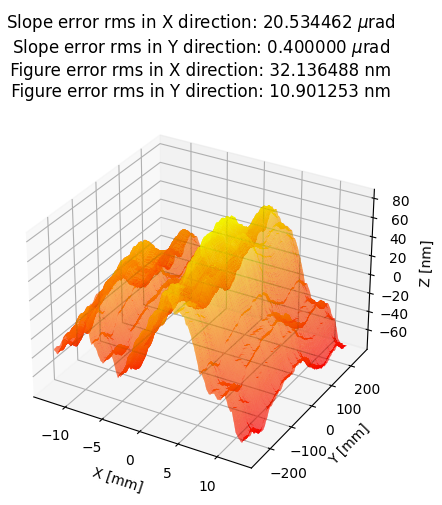
\includegraphics[width=\linewidth]{./../figures/slope_error/surface_error_profile_500x25_04x20urad.png}
  %\caption{A really Awesome Image}\label{fig:awesome_image3}
\endminipage
\caption{\label{fig:fractals} Modified mirror surfaces. }
\end{figure}
